\chapter{Конструкторский раздел}

% В данном разделе проводиться требования к разработке метода для устранения размытия на изображениях, программное обеспечение для его применения далее рассмотривается основнные моменты разработки метода и программного обеспечения для устранения размытия на изображениях.

\section{Требования к разрабатываемому методу}

При разработке метода для устранения эффекта размытия на изображениях с использованием нейронных сетей необходимо учесть следующие требования:

\begin{enumerate}[left=0.49cm]
    \item Метод должен поддерживать загрузку изображений в различных форматах для обеспечения удобства пользователя.

    \item Эффективное устранение размытия, сохраняя при этом детали и качество изображения, а также восстановление четкости и резкости краев объектов на изображении.

    % \item Результаты работы метода должны быть визуально представлены пользователю для оценки эффективности, а также проведена оценка качества работы метода с использованием объективных метрик, таких как PSNR и SSIM.

    \item Метод должен использовать нейронные сети для эффективного обучения на больших объемах данных и выявления сложных закономерностей в изображениях, которые должны быть специально адаптированы для задачи устранения размытия.
\end{enumerate}

\section{Требования к программному Обеспечению}

При разработке программного комплекса, взаимодействующего с методом устранения размытия на изображениях, необходимо учесть следующие требования:

\begin{enumerate}[left=0.49cm]
    \item Пользователь должен иметь возможность легко загружать изображения в программу через коммандную строку.

    \item После применения метода устранения размытия необходимо представить пользователю восстановленное изображение.
\end{enumerate}

% На рисунке (\ref{fig:use-case}) представлено, диаграмма вариантов использования программного обеспечения: 
% \begin{figure}[H]
% 	\centering
% 	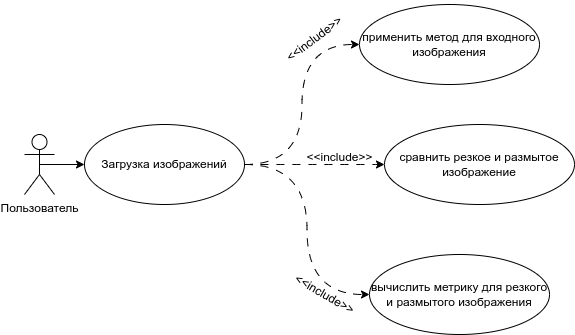
\includegraphics[width=0.5\linewidth]{assets/use-case-diagram.png}
% 	\caption{Диаграмма вариантов использования программного обеспечения}
% 	\label{fig:use-case}
% \end{figure}


\section{Требования к корпусы данных}

Корпусы данных в работе метода играет главную роль, так как будщие работы метода будет относиться к ними, требования к корпусам данных для обучения метода устранения размытия на изображениях с использованием нейронных сетей могут быть следующими:

\begin{enumerate}[left=0.49cm]
    \item Корпус данных должен включать в себя широкий спектр изображений различных типов и содержания, чтобы метод был адаптирован к различным сценариям использования и обеспечивал разнообразие изображений.

    \item Данные должны представлять изображения с различными уровнями размытия, чтобы обученная модель была способна эффективно устранять размытие в различных условиях и обеспечивала разнообразие уровней размытия.

    % \item Изображения должны иметь различные размеры и разрешения, чтобы модель была способна обрабатывать изображения различных форматов и разрешений, обеспечивая разнообразие размеров и разрешений изображений.

    \item Корпус данных должен быть разделен на независимые обучающую, валидационную и тестовую выборки для эффективного обучения, валидации и оценки модели.
\end{enumerate}

\section{Проектирование метода устранение размытия на изображениях}

\subsection{Выбор метода устранение}

Судя по перечисленным требованиям по устранению размытия на изображениях и проведенному сравнению по критериям в таблице \ref{tab:comparison}, метод MPRNet является наиболее подходящим для этой цели. Данный метод успешно справляется с задачами восстановления изображений, и его следует спроектировать таким образом, чтобы его можно было удобно обучать на различных видах изображений и чтобы он удовлетворял всем предъявляемым к нему требованиям.

Дополнительно к этому необходимо разработать пользовательский интерфейс, который позволит пользователям удобно работать с обученными нейросетевыми моделями и будет соответствовать всем перечисленным требованиям к программному обеспечению.

\subsection{Предварительная обработка изображения}

При описании MPRNet изображение, которое подается на вход в сеть, должно быть разделено на 4 равных участков. Следовательно, чтобы у пользователя не возникало проблем с загрузкой изображений разного разрешения, необходимо предусмотреть предварительную обработку изображения. Это включает дополнение изображения нулевыми пикселями перед его подачей в сеть, а затем удаление этих нулевых пикселей и представление изображения в исходном разрешении после получения результата от сети.


\subsection{Схема работы нейросети}

Перед использованием модели необходимо её обучить. Обучение сети происходит в трех режимах:

\begin{enumerate}[left=0.49cm]
	\item обучение;
	\item валидация;
	\item оценка.
\end{enumerate}

На этапе обучения подготавливается обучающая выборка, устанавливаются параметры сети и происходит обучение. После прохождения нескольких эпох выполняется валидация и оценка результатов. Стоит отметить, что обучение происходит только на обучающей выборке, а валидация происходит на валидационной выборке.

На рисунке \ref{fig:training-model} представлено, схема алгоритма обучения MPRNet:
\begin{figure}[H]
	\centeringы
	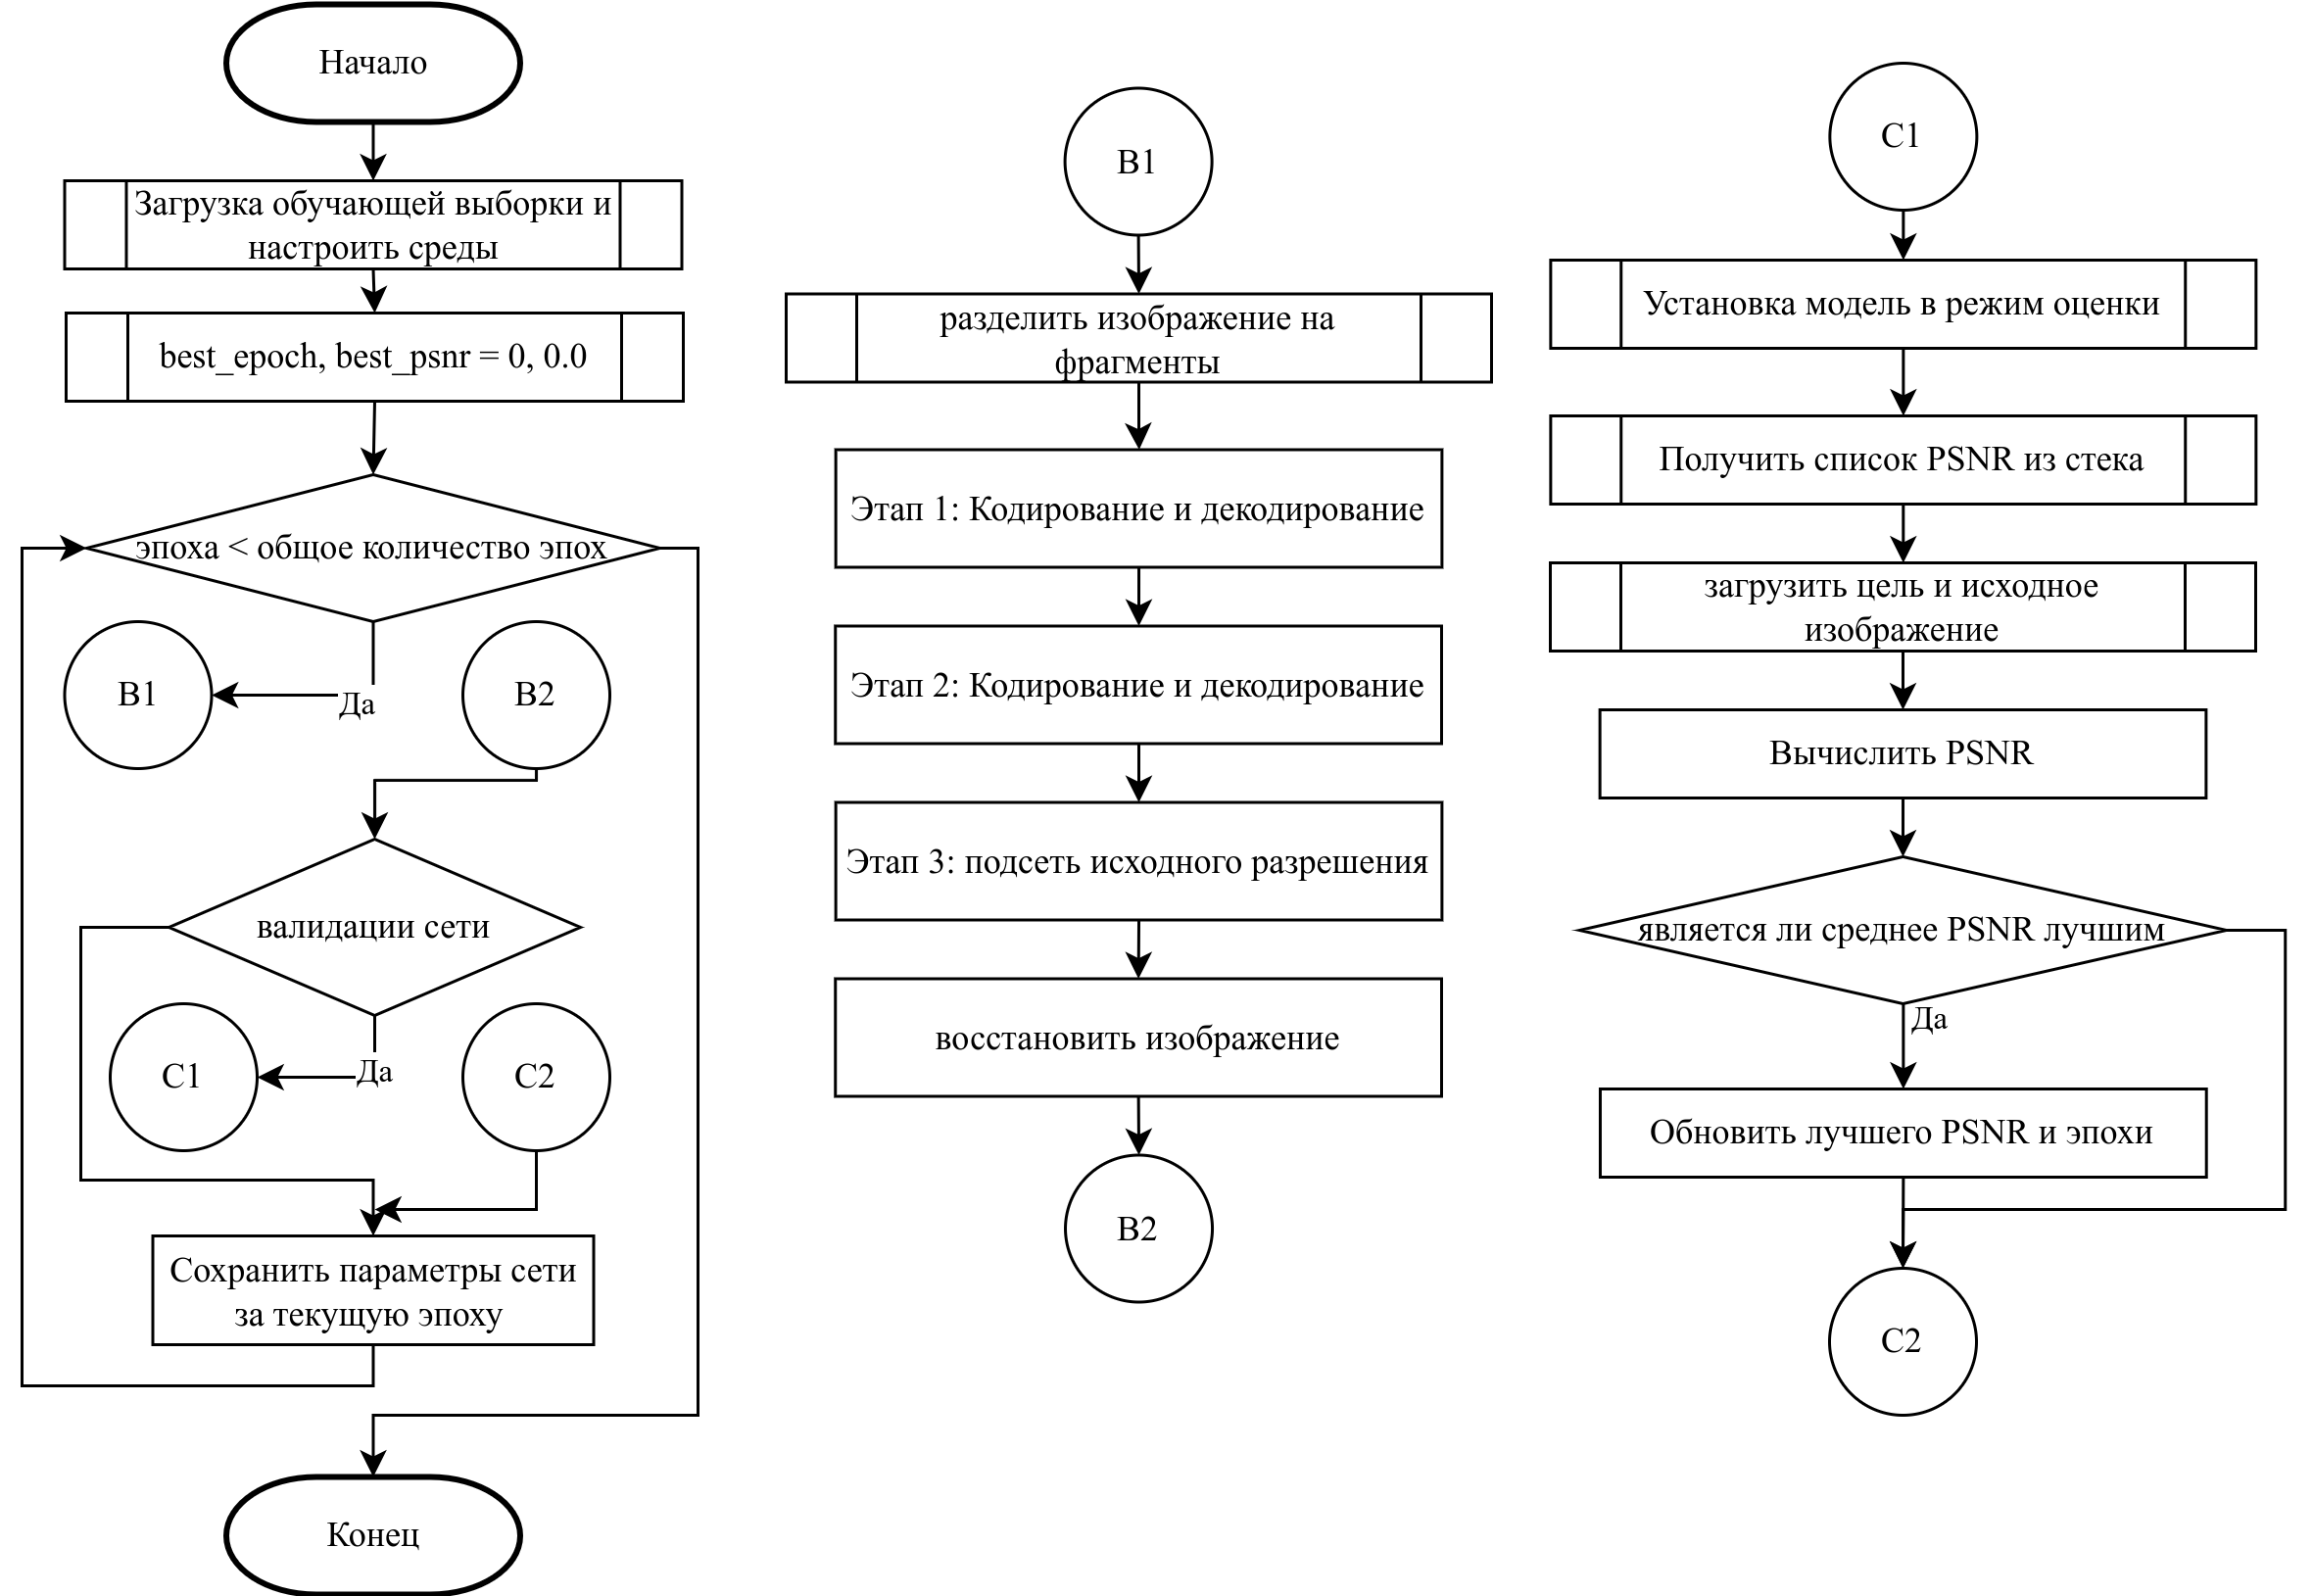
\includegraphics[width=1.0\linewidth]{assets/train-diagram.png}
	\caption{Схема алгоритма обучения MPRNet}
	\label{fig:training-model}
\end{figure}

После успешного обучения и валидации необходимо сохранить параметры сети для последующей оценки. Для оценки работы сети по устранению изображений необходимо провести оценку на некотором наборе изображений, которые не использовались в процессе обучения и валидации.

На рисунке \ref{fig:predict-model} представлено, схема работы программного обеспечения в режиме оценки:
\begin{figure}[H]
	\centering
	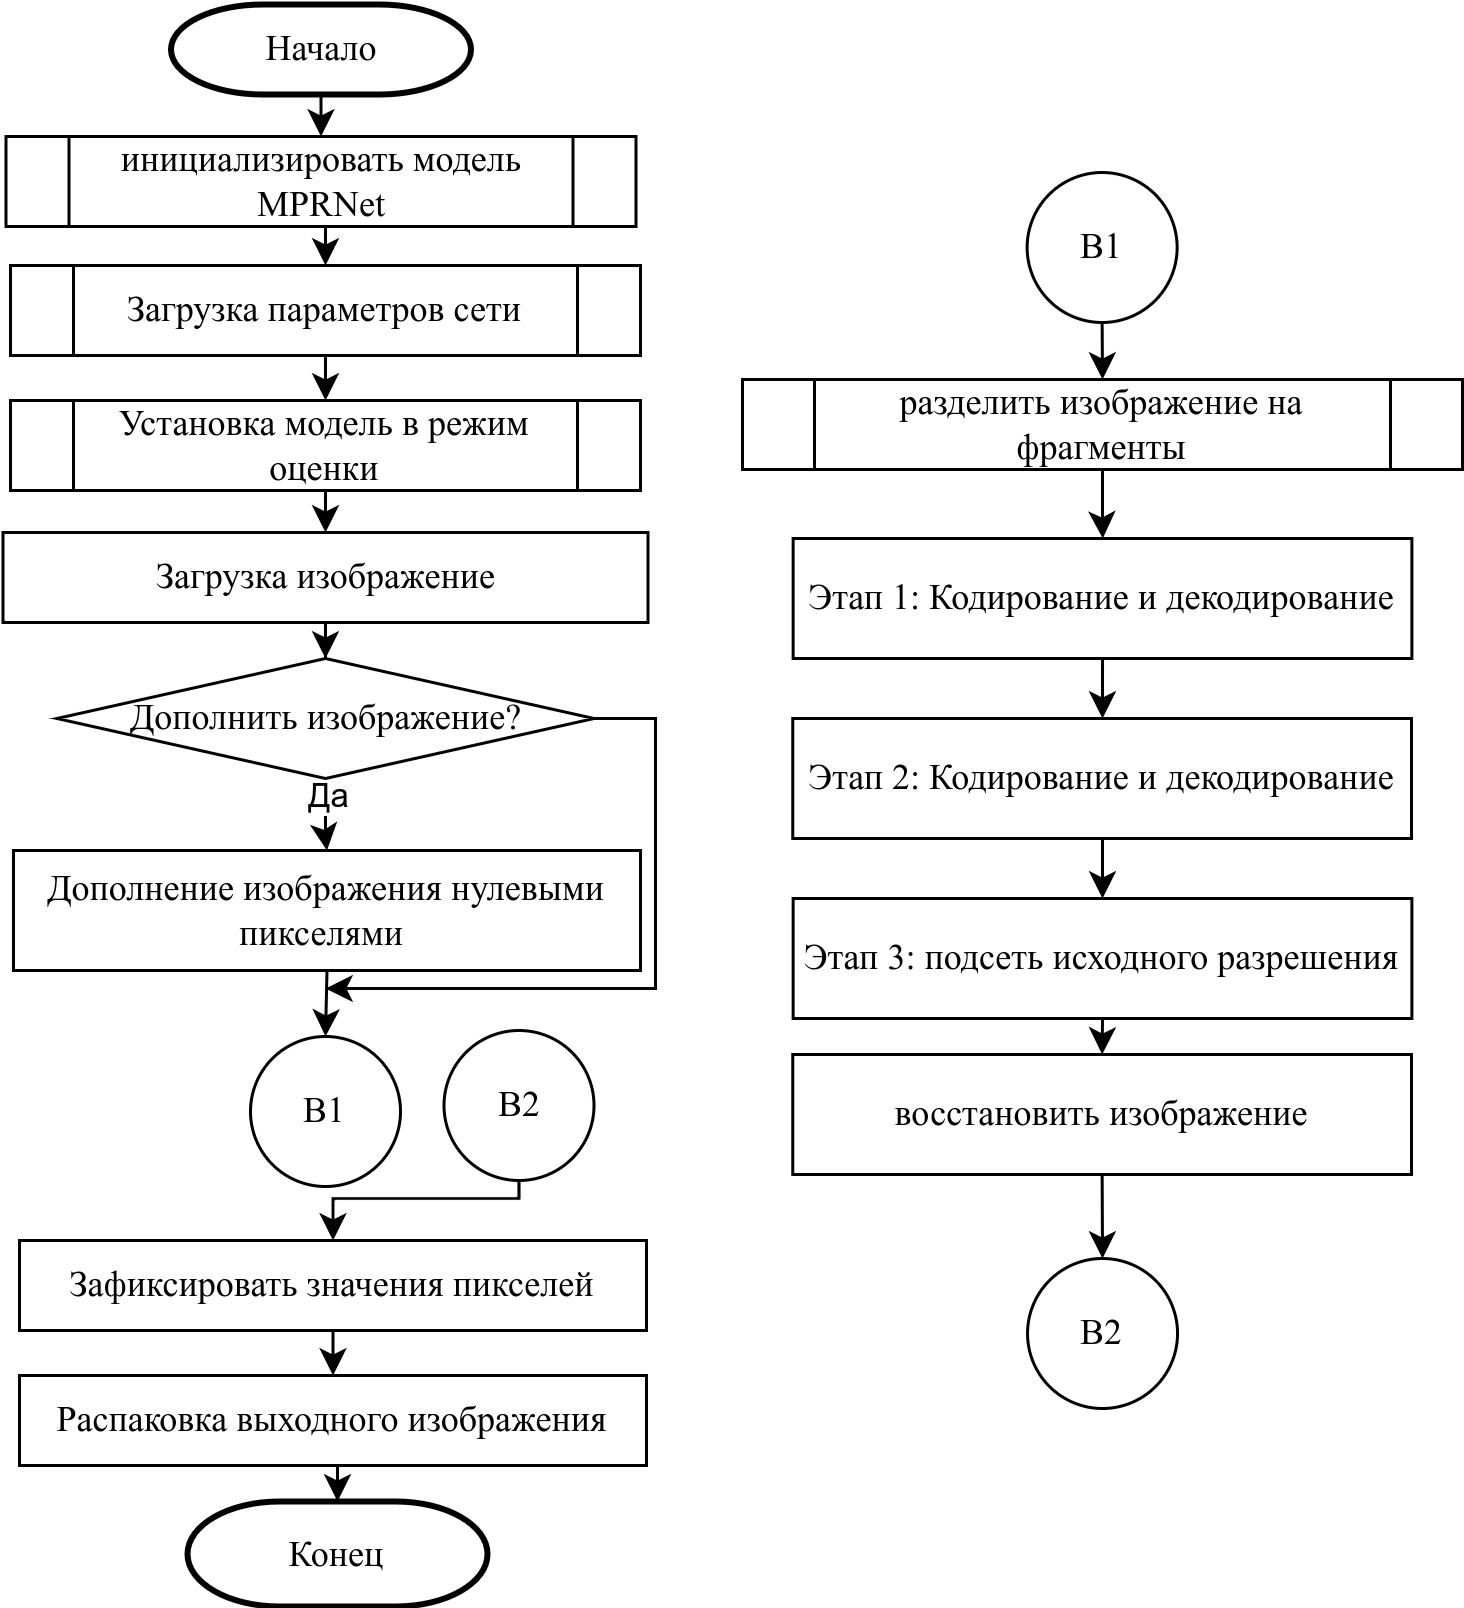
\includegraphics[width=1.0\linewidth]{assets/predict-diagram.png}
	\caption{Схема работы программного обеспечения в режиме оценки}
	\label{fig:predict-model}
\end{figure}

\subsection{Структура разрабатываемого программного обеспечения}

Будущее программное обеспечение должно работать в двух режимах: режиме обучения и режиме оценки. В режиме обучения пользователь должен иметь возможность задавать параметры обучения нейросетевой модели через файл и конфигурации. Модель должна получать информацию о местонахождении выборок для обучения, валидации и тестирования из указанных файлов. В режиме оценки программа должна представлять все вышеуказанные требования.

На рисунке \ref{fig:training-model} представлено, схема работы программного обеспечения в режиме обучения:
\begin{figure}[H]
	\centeringы
	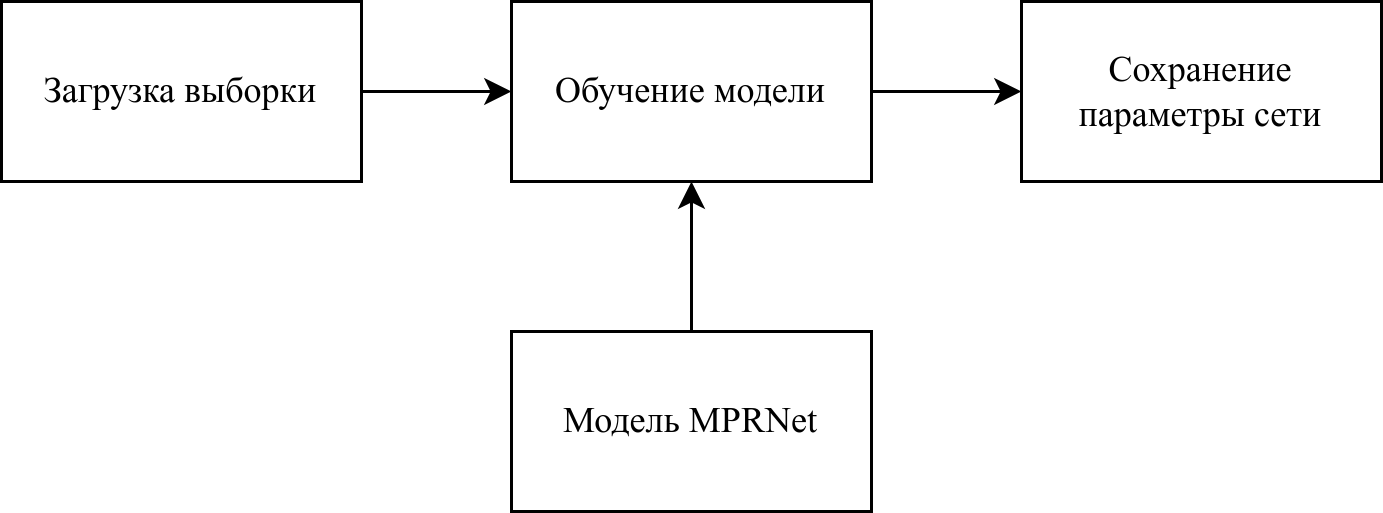
\includegraphics[width=1.0\linewidth]{assets/training-model.png}
	\caption{Схема работы программного обеспечения в режиме обучения}
	\label{fig:training-model}
\end{figure}

На рисунке \ref{fig:predict-model} представлено, схема работы программного обеспечения в режиме оценки:
\begin{figure}[H]
	\centering
	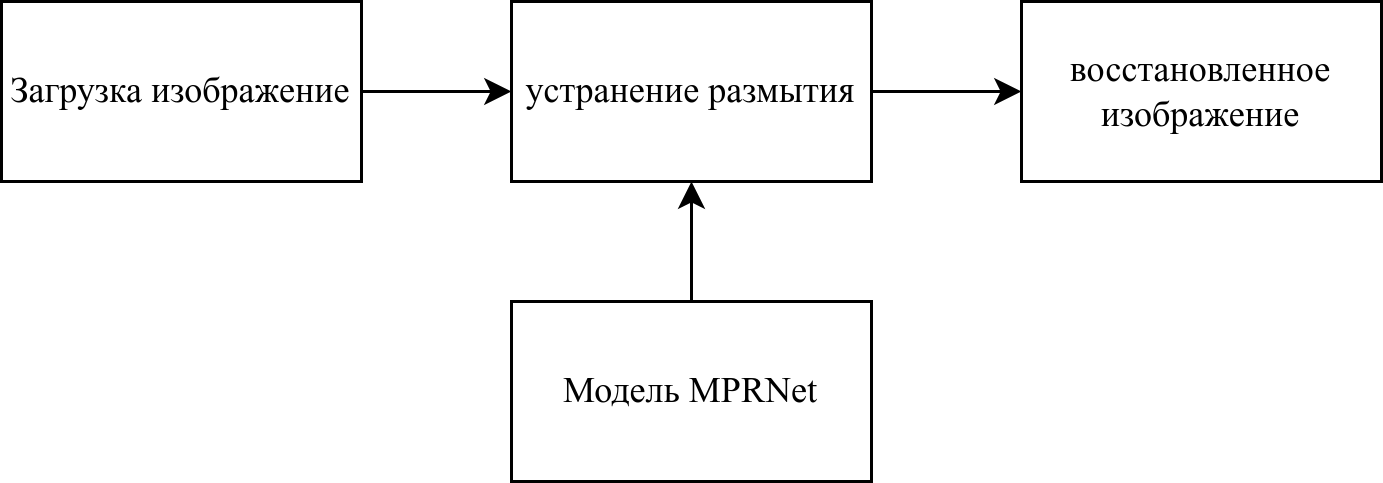
\includegraphics[width=1.0\linewidth]{assets/predict-model.png}
	\caption{Схема работы программного обеспечения в режиме оценки}
	\label{fig:predict-model}
\end{figure}

\section{Корпусы данных}

Задачей, представленной в данной выпускной квалификационной работе, является устранение размытия на изображениях. Судя по требованиям, изображения, которые будут участвовать в обучении сети, должны содержать контент с несколькими людьми, а также изображения, на которых присутствует только один человек, и изображения, на которых людей нет. Далее следует разделить данные для эффективного обучения нейросетевых архитектур на три выборки:
\begin{enumerate}[left=0.49cm]
    \item обучающую;
    \item валидационную;
    \item тестовую.
\end{enumerate}

Корпус данных GoPro \cite{nah2017deep} и корпус данных HIDE \cite{shen2019human} содержат в себе примеры изображений с различными уровнями размытия. Разрешение изображений в обоих корпусах составляет 1280x720 пикселей. Изображения из этих двух корпусов соответствуют установленным требованиям по контенту. Количество изображений в корпусе данных GoPro составляет 3214 пар, а в корпусе HIDE - 2025 пар, которые соответствуют требованиям по теме данной работы.

На рисунке \ref{fig:dataset-example} представлено, пример изображение из корпуса данных:
\begin{figure}[H]
	\centering
	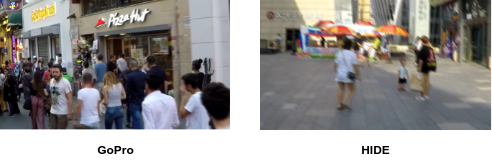
\includegraphics[width=0.75\linewidth]{assets/dataset-example.png}
	\caption{Пример изображение из корпуса данных}
	\label{fig:dataset-example}
\end{figure}

\section*{Вывод}

В данном разделе были рассмотрены требования к разработке метода, программному обеспечению и корпусам данных, было представлено описание программы в обучающем режиме и в режиме оценки. Была представлена информация о корпусах данных, соответствующих перечисленным требованиям, проведено описание основных моментов разработки сети и алгоритмов, которые необходимо учитывать при разработке.